\chapter{Monte Carlo-Daten}

Ein großes Ziel in der Astroteilchenphysik ist es, Aussagen über die Energiespektren von astrophysikalischen Quellen zu machen.

In der Cherenkovastronomie sind dafür Monte Carlo (MC)-Daten von grundlegender Bedeutung:
Für die Rekonstruktion eines Energiespektrums einer Gamma-Quelle müssen zunächst einmal Signalevents, die aus der Quelle kommen und Background-Events voneinander getrennt werden.
Dies geschieht heutzutage mit künstlichen Lernalgorithmen, die auf wohl bekannten Beispieldaten, den MC-Daten, trainiert werden müssen.
Auch für die Methode der Entfaltung des Energiespektrums werden MC-Daten benötigt.

Die komplette Produktion der MC-Daten für das MAGIC Experiment wurde im Rahmen dieser Doktorarbeit durchgeführt und wird in diesem Kapitel detailliert beschrieben.

Es werden zunächst die Programme beschrieben, die in der MAGIC MC - Simulationskette und später in der Kalibrationskette genutzt werden.
Angefangen mit der Simulation der Luftschauer mit \textit{CORSIKA} über die Reflektor- und die Kamera-Simulation bis zur Berechnung der Bildparameter des bereinigten Events wird hier alles beschrieben.
Dabei bauen die Simulationsschritte aufeinander auf, sodass die simulierten Corsika-Events bis zum letzten Schritt weiter prozessiert werden.

Für die eigentlichen Simulationsprogramme (\textit{CORSIKA}, \textit{Reflector} und \textit{Camera}) wird jeweils eine Übersicht über einige wichtige Inputparameter, die den Programmen als text-Dateien,
sogenannten Inputcards, übergeben werden, gegeben.
Nach Abschluss der Simulationskette liegen dann die MC Daten in der gleichen Form vor wie die aufgenommenen Daten der Teleskope. 
Die anschließenden Schritte der Kalibrationskette (\textit{Sorcerer}, \textit{Star} und \textit{Superstar}) werden ebenfalls beschrieben.
Diese Kalibration wird im MAGIC Datenzentrum genauso mit den real aufgenommenen Daten durchgeführt, sodass am Ende alle Daten (reale und simulierte) im gleichen Format vorliegen.

Nachdem alle Programme zur Simulation und Kalibration erklärt wurden, wird auf die automatische Produktionsstruktur auf dem Rechencluster LiDO an der TU Dortmund eingegangen.

% \vspace{\fill}
\section{Schauersimulation mit CORSIKA}

CORSIKA wurde am Forschungszentrum Karlsruhe ursprünglich für das KASCADE-Experiment entwickelt und wird heute in vielen Astroteilchenexperimenten eingesetzt.
Mit \textit{CORSIKA} werden ausgedehnte Luftschauer, ausgelöst von kosmischer Strahlung simuliert.

Es können verschiedene Primärteilchen wie Protonen, Eisenkerne oder Photonen als Primärteilchen eingestellt werden.
Diese Primärteilchen werden durch die Atmosphäre propagiert, wo sie Wechselwirkungen mit den Kernen der Luft eingehen und Schauer produzieren oder aber zerfallen.
Die entstandenen Schauer werden dann bis zum Teleskop simuliert.


% \begin{figure}
%     \centering
%     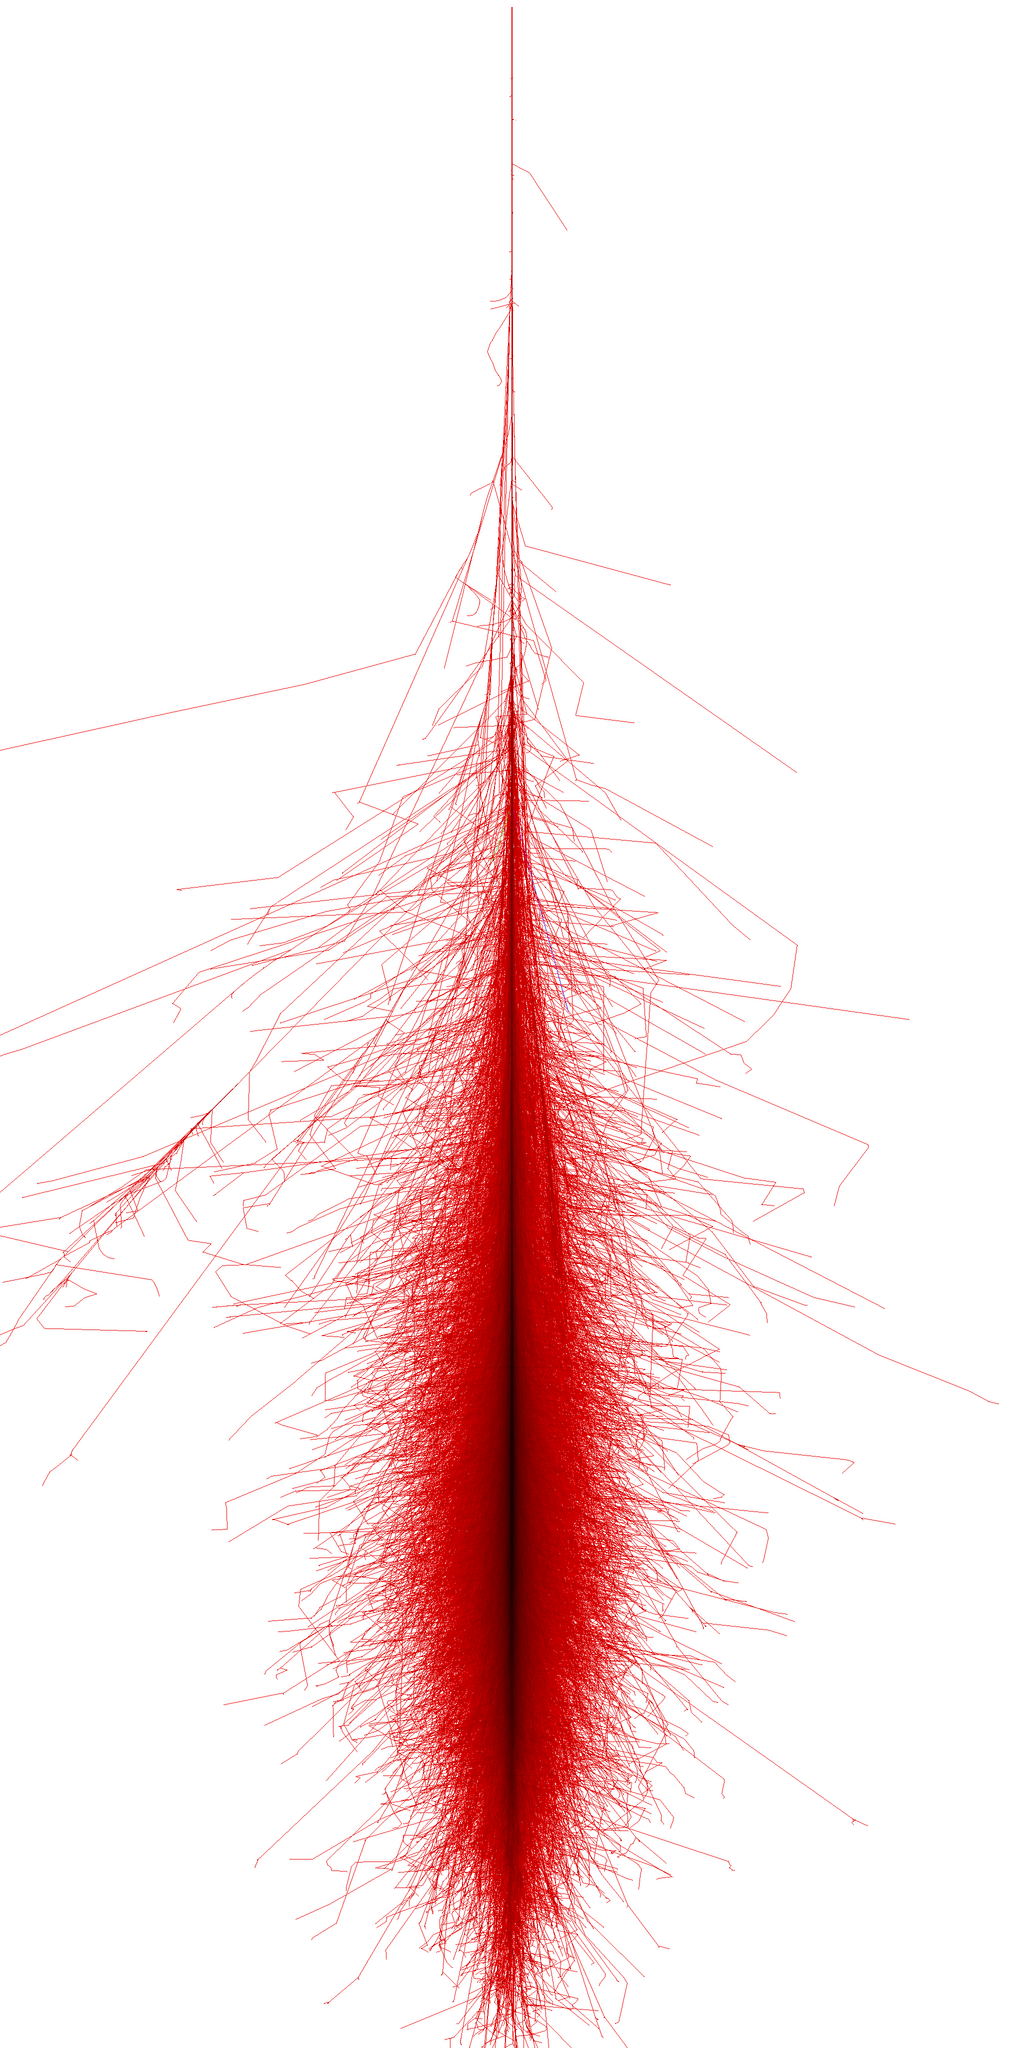
\includegraphics[width=0.3\textwidth]{./Plots/Photon_1TeV_CORSIKA.png}
%     \caption{Schematische Darstellung der automatischestionskette.}
%     \label{CORSIKA_Photon}
% \end{figure}

\begin{figure}
 \begin{subfigure}{0.4\textwidth}
  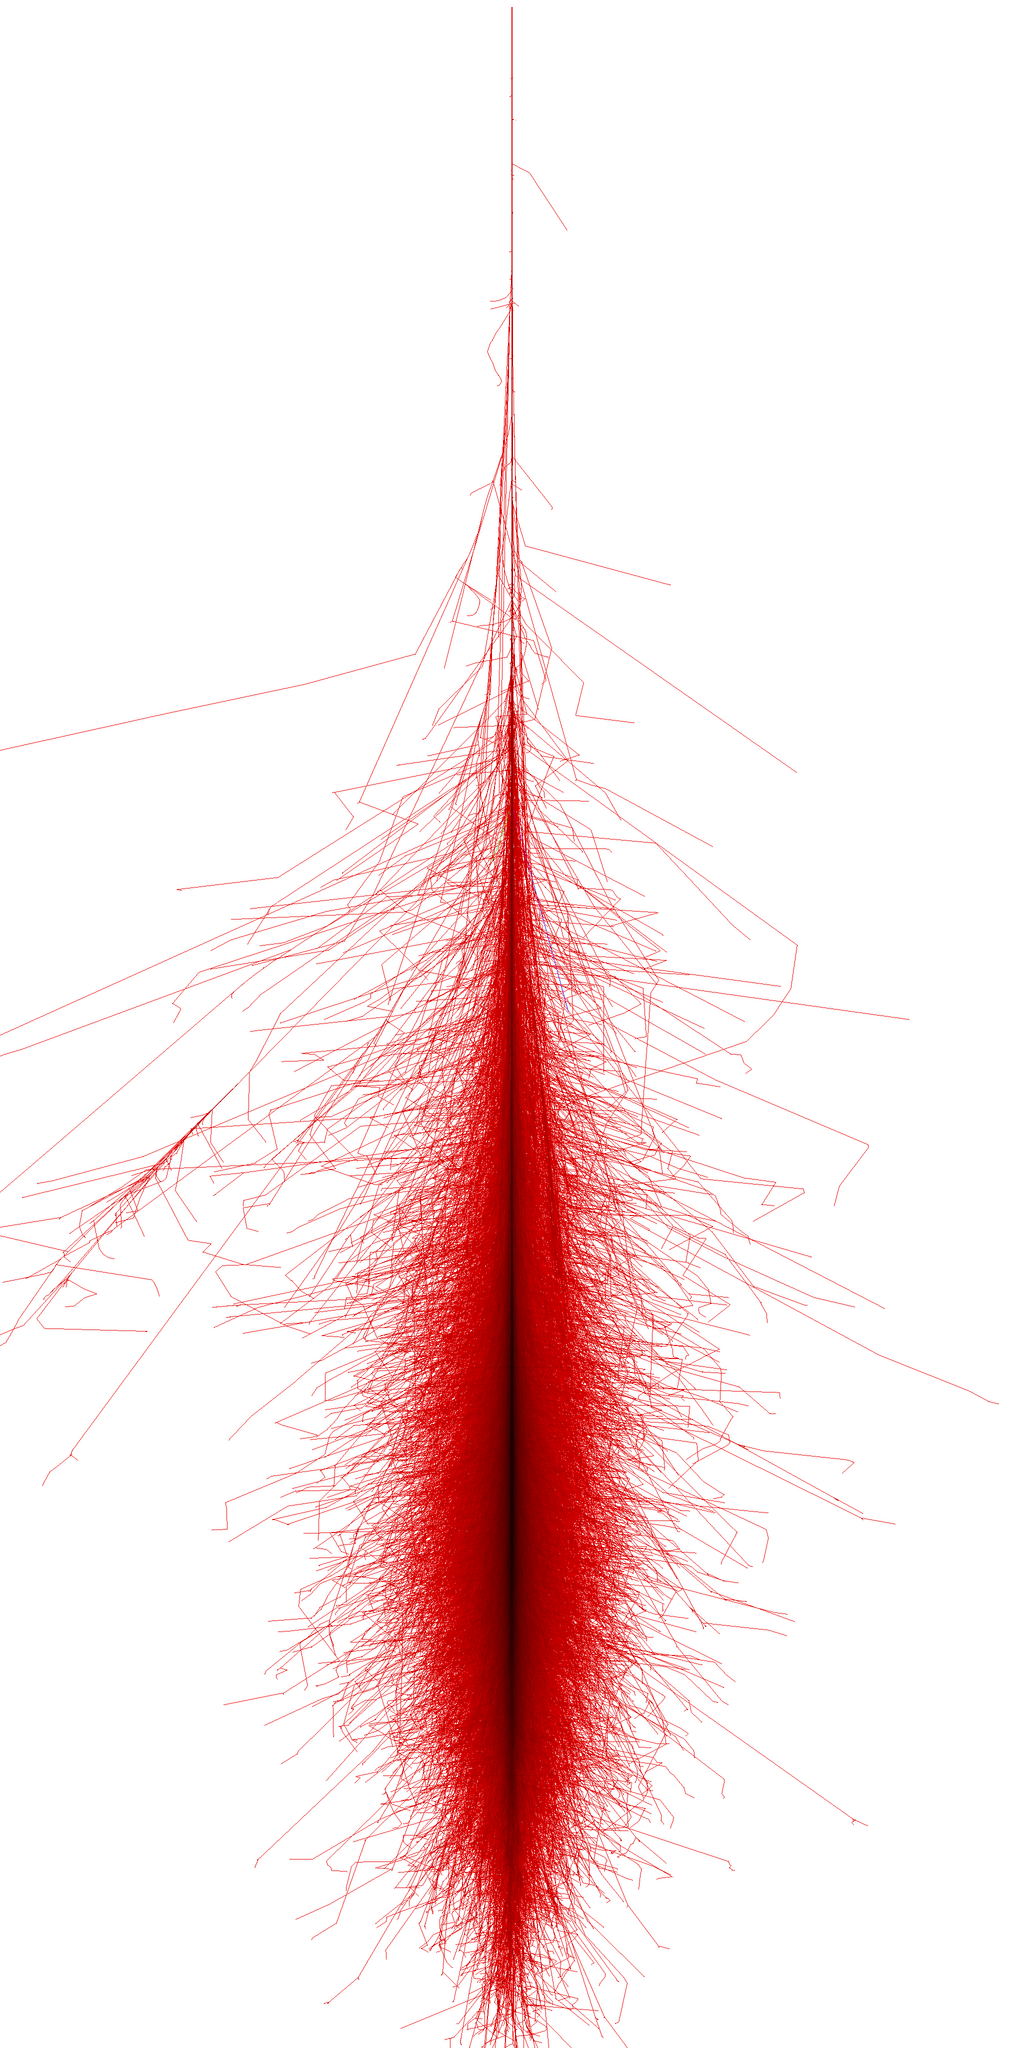
\includegraphics[width=\textwidth]{./Plots/Photon_1TeV_CORSIKA.png}
  \caption{Simulation eines Schauers mit 1TeV-Photon als Primärteilchen}
 \end{subfigure}
 \hspace{2.0cm}
  \begin{subfigure}{0.4\textwidth}
  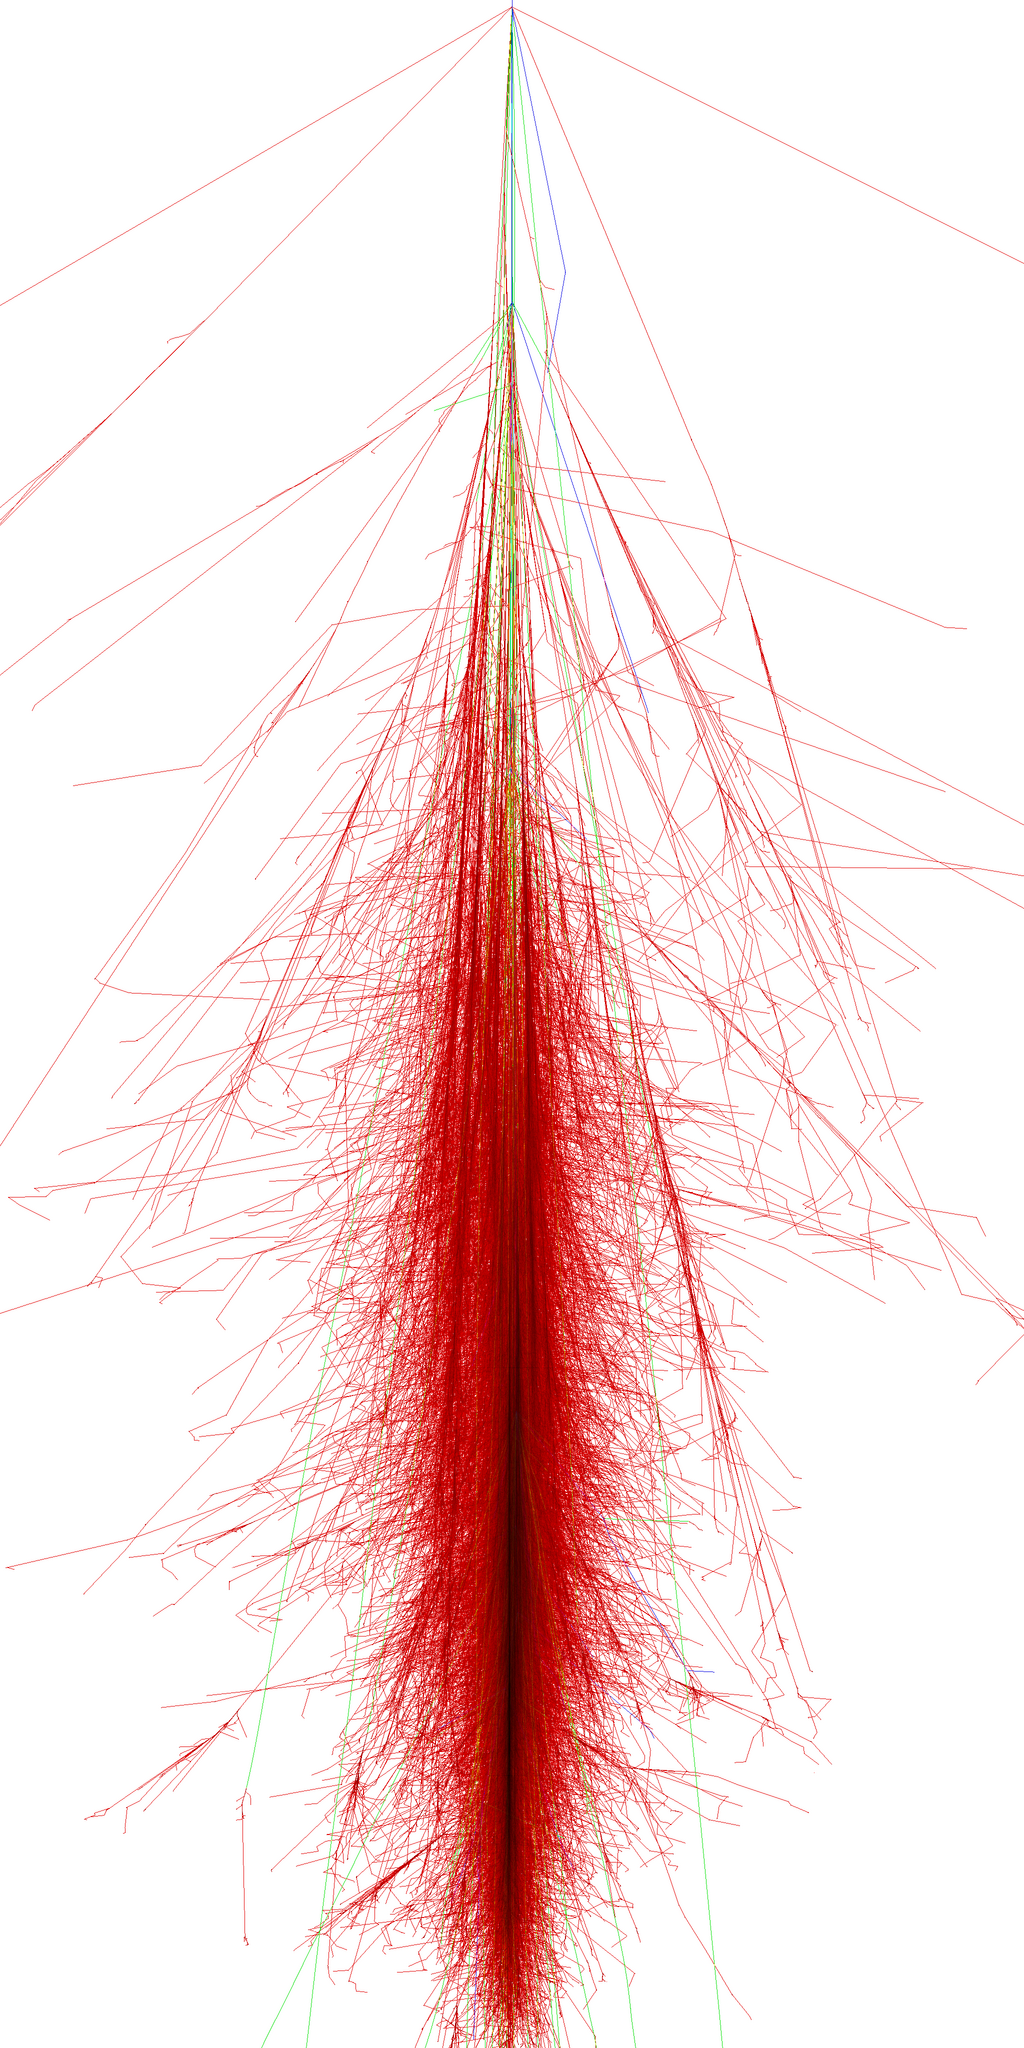
\includegraphics[width=\textwidth]{./Plots/Proton_1TeV_CORSIKA.png}
  \caption{Simulation eines Schauers mit 1TeV-Proton als Primärteilchen}
 \end{subfigure}
  \caption{ Schauersimulation mit CORSIKA mit 1TeV Primärteilchen}
  \label{CORSIKA_Schauer}
 \end{figure}



In Abb.\ref{CORSIKA_Schauer} sieht man die verschiedenen Eigenschaften der Schauer: Hadronische Schauer haben einen größeren Querschnitt und sind weniger kompakt verglichen mit elektromagnetischen.

Es sind verschiedene Modelle für die hadronische Wechselwirkung bei hohen Energien und bei niedrigen Energien implementiert.
Für die MAGIC MC-Simulation werden QGSJET II für die hadronische Wechselwirkung bei hohen Energien und FLUKA für die Wechselwirkung bei niedrigen Energien benutzt.
Elektromagnetische Prozesse werden mit dem EGS4-Modell beschrieben.
Eine Simulation der Cherenkovphotonen, die von den geladenen Teilchen produziert werden, die durch die Luft propgaieren, erfolgt ebenfalls.

\subsection{Mmcs}
Eine speziell für das MAGIC-Teleskop adaptierte Version von \textit{CORSIKA} wird in der Standardsimulation genutzt.
In dieser Version wurde der Einfluss des Magnetfeldes vor der ersten Wechselwirkung auf das Primärteilchen vernachlässigt um zu verhindern, dass es zu weit vom Teleskop abgelenkt wird.
Außerdem wurde die Simulation der Cherenkovwellenlänge eingebaut und es wurde eingebaut, dass alle Informationen über das Primärteilchen gespeichert werden.

\subsection{Inputcards}
Die Inputcard enthält Informationen über den Teleskopstandort, die simulierten Schauer und über das Magnetfeld.

Zunächst können allgemeine Angaben zur Anzahl der simulierten Events gemacht werden. 
So erhält jeder \textit{CORSIKA}-Run eine eigene Runnumer und die Anzahl der Schauer pro Run wird durch den Parameter \texttt{NSHOW} angegeben.

Außerdem erfolgen noch Einstellungen über die Eigenschaften der Schauer.
Der Parameter \texttt{PRMPAR} gibt die Art des Primärteilchens an und \texttt{ERANGE} beschreibt den Energiebereich, in dem die Primärteilchen simuliert werden.
Die Steigung des Energiespektrums wird mit dem Parameter \texttt{NSLOPE} eingestellt.
Zenit- und Azimutbereich, in dem die Schauer simuliert werden, wer den durch \texttt{THETAP} und \texttt{PHIP} angegeben.

Zudem werden in \textit{CORSIKA} noch Standortangaben zur Geographie des Teleskopstandortes gemacht.
So wird die Höhe über NN im Parameter \texttt{OBSLEV} angegeben und eine Angabe über die horizontale, bzw. vertikale Komponente des Magnetfeldes auf La Palam befindet sich im Parameter \texttt{MAGNET}.
Der Parameter \texttt{ATMOSPHERE} gibt an, welche Parametrisierung der Atmosphäre genutzt wird.

Abgesehen von diesen allgemeinen Angaben gibt es in der Inputcard noch einige Parameter, die dediziert für die Simulation der Cherenkovphotonen sind.
Der Wellenlängenbereich, in welchem Cherenkovphotonen simuliert werden, wird mit \texttt{CWAVLG} angegeben.
Der Impact-Parameter, der angibt, in welcher Entfernung der Schauer vom Teleskop entfernt auftreffen kann, wird mit \texttt{CSCAT} angegeben.
Der Parameter \texttt{CERTEL} beinhaltet Standort und Größe der Teleskope, die man simuliert und mit der Option \texttt{CERFIL} wird angegeben, ob der Output über die Cherenkovphotonen in eine extra Datei geschrieben wird.


% Einige Einstellungen werden im Folgenden beschrieben:
% 
% \begin{itemize}
%  \item Jedem Corsika-Run wird eine eigene Runnummer zugewiesen
%  \item Mit PRMPAR wird die Art des Primärteilchens eingestellt, was simuliert werden soll.
%  \item ERANGE beschreibt den Energiebereich, in dem Primärteilchen simuliert werden.
%  \item Die Anzahl der Schauer pro Run wird durch NSHOW angegeben.
%  \item Es ist möglich, den Slope des Energiespektrums der Primärteilchen mit ESLOPE einzustellen.
%  \item THETAP und PHIP beschreiben den Zenit- und Azimutbereich, in dem die Schauer simuliert werden.
%  \item Die Höhe über NN des Teleskops wird mit OBSLEV angegeben.
%  \item MAGNET gibt die horizontale und die vertikale Komponente des Magnetfeldes auf La Palma an.
%  \item ECUTS sind die Cut-offs in der unteren Energie für Hadronen, Myonen, Elektronen und Photonen.
%  \item MUADDI gibt falls es auf TRUE gesetzt schreibt zusätzliche Informationen über Myonen raus.
%  \item Mit MUMULT kann man einstellen auf welche Art die Myonen gestreut werden.
%  \item LONGI ist ein Parameter für die longitudinale Schauerentwicklung.
%  \item MAXPRT ist die maximale Nummer der gedruckten Events.
% \end{itemize}
% 
% Nun gibt es in der INputcard noch einige Parameter die dediziert für die Simulation der Cherenkovphotonen sind:
% So zum Beispiel:
% 
% \begin{itemize}
%  \item CWAVLG gibt an, in welchem Wellenlängenbereich Cherenkovphotnen simuliert werden sollen.
%  \item Mit CSCAT kann man einstellen, wie oft ein Cherenkovevent wiederbenutzt wird und der Impact ,d.h. der Bereich, in dem der Schauercore vom Teleskop entfernt auftreffen kann.
%  \item Falls CERFIL TRUE ist, wird der Output über die Cherenkovphotonen in ein extra File geschrieben.
%  \item Mit CERTEL gibt man den Standort und die Größe der Teleskope an, für die man simulieren möchte.
%  \item ATMOSPHERE sagt, welche Parametrisierung der Atmosphäre genutzt werden soll.
% \end{itemize}

\section{Simulation des Reflektors mit Reflector}
Wie der Name schon sagt, wird im Programm \textit{Reflector} vor allem der Reflektor simuliert, allerdings kommen noch einige Zusatzfunktionen ins Spiel.

Mit \textit{Reflector} wird zuerst die atmosphärische Absorption der Cherenkovstrahlung in der Luft simuliert. 
Dabei werden Rayleigh-Streuung, Mie-Streuung und die Absorption an Ozon simuliert.
Als nächstes wird mit Hilfe von Ray-Tracing simuliert, ob die Cherenkovphotonen den Teleskopspiegel treffen.
Dort angekommen muss die Absorption der Aluminium-, bzw. Glasspiegel berücksichtigt werden und die Photonen reflektiert werden.
Nach der Reflexion am Spiegel wird nacheinander überprüft, ob die Photonen die Kamera treffen und letztendlich die Ankunftszeiten in der Kamera bestimmt.

\subsection{Inputcards}
Für diese Simulationsschritte werden bestimmte Inputparameter, bzw. Inputdateien benötigt, die die Eigenschaften des Reflektors beschreiben.
Die wichtigsten werden im Folgenden kurz erklärt.

Es muss der Pfad zur \textit{CORSIKA}-Inputdatei sowie die Output-Pfade für die beiden Reflektordateien (je eine pro Teleskop) angegeben werden.

Teleskopstandort und Wobble Position müssen angegeben werden.

Pro Teleskop wird ein \texttt{mirror\_definition\_file} für die verschiedenen Spiegel (Glas und Aluminium) benötigt.
In dieser Datei sind grundlegende Eigenschaften des Teleskops wie zum Beispiel der Abstand zwischen Spiegel und Kamera festgelegt. 
Des Weiteren wird der Kameraradius angegeben und die Anzahl der Spiegel mit ihrer jeweilige Größe.
Für jeden Spiegel sind einzeln ihre jeweilige ID, der Fokalabstand, die Koordinaten des Spiegelmittelpunkts und der Normalenvektor des Spiegels aufgelistet.

Im sogenannten \texttt{reflectivity\_file} sind die gemessenen Reflektivitäten der einzelnen Spiegel aufgelistet.

Das \texttt{axisdev\_file} beschreibt die Abweichung der einzelnen Spiegel von der idealen Pointing Position.

Im \texttt{measuredpsf\_file} ist die gemessene PSF eingetragen.

Letztendlich muss man in Reflector noch das Atmosphärenmodell, welches für die Simulation benutzt werden soll, angegeben werden. 
Aktuell wird das MagicWinter-Modell benutzt. 
Eine Parametrisierung des Modells enthält abhängig von der Höhe die Dichte, die Dicke und der Brechungsindex (siehe Arbeit von Mareijke Haffner).


\section{Simulation von Kamera und Elektronik mit Camera}
Das Programm \textit{Camera} simuliert das komplette Verhalten der Kamera inklusive der Beiträge des Nachthimmeluntergrundes (NSB).
Es werden neben den Schauern also auch der diffuse NSB und Sterne im Field of View simuliert. 
Des Weiteren werden der Trigger und das elektronische Rauschen simuliert, sodass bei einer Änderung der Hardware der Kamera, bzw der Elektronik nicht die komplette MC Kette noch einmal durchlaufen werden muss.
In Abb.\ref{Kamera-Bild} befindet sich ein generiertes Cherenkovevent in der Kamera mit einer Energie von $\SI{3.0}{TeV}$.

\begin{figure}
    \centering
    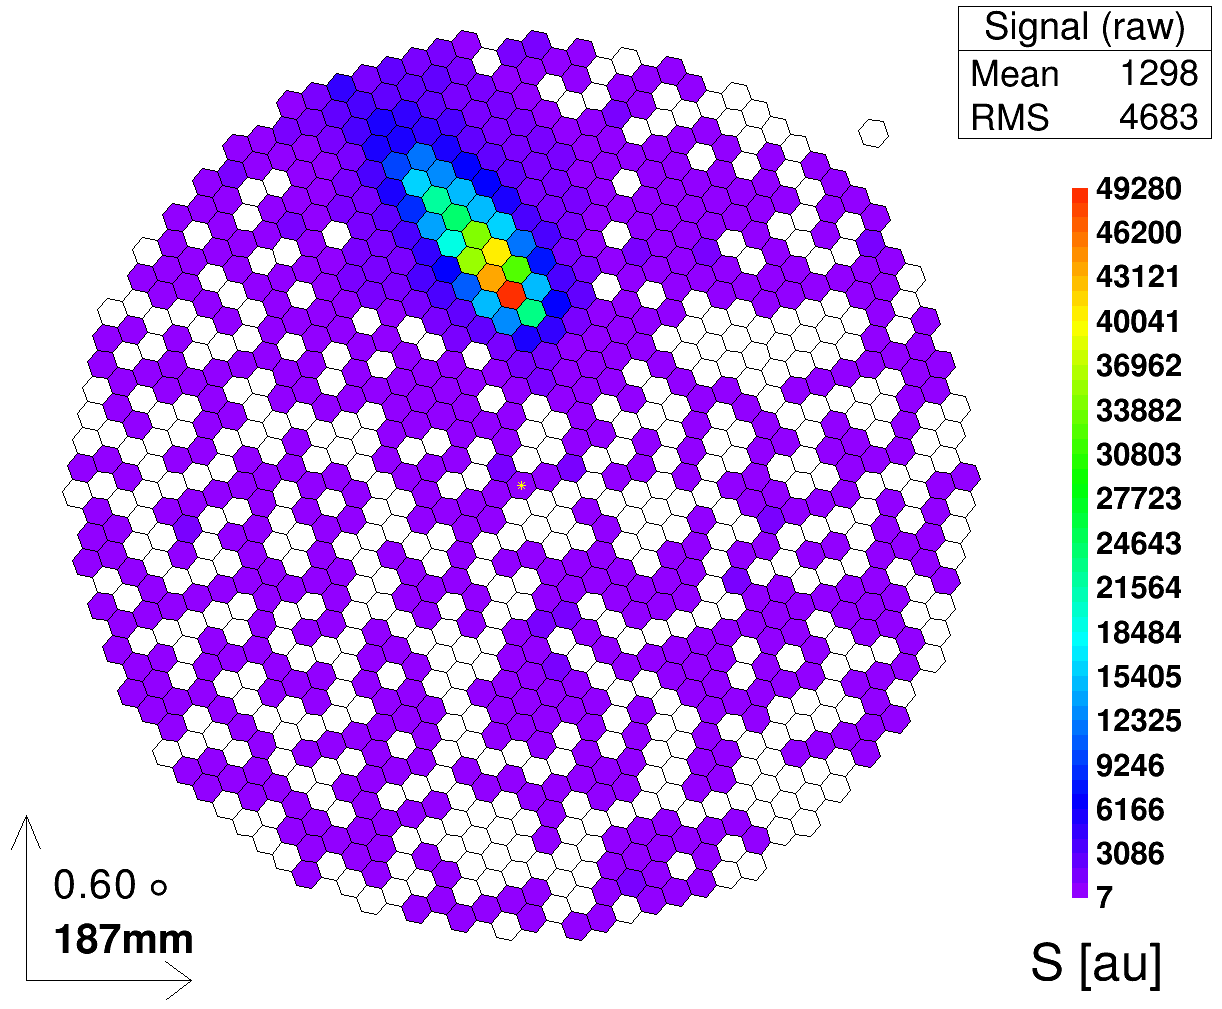
\includegraphics[width=0.6\textwidth]{./Plots/Signal_Job481_RunNr1513276_511_e3.0TeV_Zd32.2_fertig.png}
    \caption{Darstellung eines simulierten Schauers mit einer Primärteilchenenergie von $\SI{3.0}{TeV}$ in der Kamera. Dargestellt ist der Pixelinhalt in [a.u.].}
    \label{Kamera-Bild}
\end{figure}

Im Folgenden wird die Simulation beschrieben, die mit zwei möglichen vorbereitenden Schritten beginnt: der Simulation des NSB und der Sterne im FoV.

\subsection{StarFieldAdder und StarResponse}
Da MAGIC sensitiv für Sterne bis zur Magnitude 10 ist, tragen die Sterne zum Rauschen in der Kamera bei.
Das Programm \textit{StarFieldAdder} berechnet anhand von einem Katalog, welche Sterne im FoV sind und berechnet dann, wieviele Photonen von diesen Sternen mit welcher Wellenlänge den Spiegel treffen.
Der Output wird im \textit{CORSIKA}-Format geschrieben und muss noch durch \textit{Reflector} laufen, bevor er von \textit{Camera} benutzt werden kann.
Eine Simulation der Sterne im FoV wird in der Standard-MC-Simulation nicht durchgeführt, da die MC-Daten für alle Quellen in einem bestimmten Zenitbereich benutzt werden sollen und nicht für jede Quelle eigene MC-Daten produziert werden.

Um die Simulation zu beschleunigen und damit nicht für jedes Event der diffuse NSB neu berechnen werden muss, wird mit \textit{StarResponse} eine NSB-Datenbank generiert und daraus dann das NSB-Rauschen berechnet, welches dann zusammen mit dem Cherenkovphotonensignal zum Trigger geht.

\subsection{Simulation von Kamera und Elektronik}
Nachdem alle Parameter aus der Inputcard eingelesen worden sind und die individuelle PixelResponse mit NSB gefüllt wurde, erfolgt die eigentliche Verarbeitung der zuvor simulierten \textit{Reflector}-Daten.
Die Photonen aus den Schauern werden eingelesen und für jedes Photon werden folgende Werte einzeln bestimmt:

\begin{itemize}
 \item Pixelization: In welchem Pixel kommt das Photon an
 \item PhE-Produktion: Unter Berücksichtigung der wellenlängenabhängigen Quanteneffizienz jedes PMTs und der Winston Cones wird entschieden, ob ein Photoelektron erzeugt wird.
 \item Channel Response: Für jedes Photoelektron, was die Photokathode verlässt, wird das Analogsignals des PMTs generiert.
\end{itemize}

Danach werden die Signale und Ankunftszeiten aller Photonen eines Pixel superponiert und die Response des Triggers und FADC Systems berechnet und elektronisches Rauschen hinzugefügt.
Das wird für alle Pixel gemacht und man erhält das analoge Signal.
Dann wird durch eine Baseline-Subtraction die AC Kopplung simuliert, die zwischen dem PMT Output und dem Signal ist, welches in den Discriminator Trigger geht.
Danach steht noch die Simulation des Triggers aus. 
Es wird gecheckt, ob das analoge Signal eine bestimmte Schwelle, die Discriminator Schwelle, überschreitet.
Falls ja, wird ein digitales Output Signal simuliert.
Dann wird der first Level Trigger simuliert:
Ob das Event triggert beruht auf seiner Topologie und der Multiplizität.
Dafür wird eine Nächste-Nachbarn-Bedingung überprüft, d.h. die minimale Anzahl an Pixeln, die einen bestimmten Photoneninhalt haben und ihre Verteilung in der Kamera.
Falls diese Bedingungen erfüllt sind, wird ein First Level Trigger Signal generiert und der Output des FADC Systems, welches die digitalisierte Form des analogen Signals ist, wird gespeichert.
Dann wird der nächste Schauer prozessiert.

\subsection{Inputcard}
Im Folgenden werden einige Parameter erklärt, die in der Inputcard von \textit{Camera} enthalten sind.
Wie in jeder Inputcard müssen die Pfade zu den zu prozessierenden \textit{Reflector}-Dateien angegeben sein sowie ein Output-Pfad.
Im Folgenden werden einige Dateien angegeben, die das Programm Camera benötigt:

\begin{itemize}
 \item \texttt{qe\_file}, in welchem die Quanteneffizienz der PMTs als Funktion ihrer Wellenlänge angegeben ist
 \item \texttt{lightcollision.dat}, was die Lichtkollektionseffizienz der Pixel als Funktion des Winkels zwischen Photontrajektorie nach der Reflexion am Spiegel und der Kameraebene angibt.
 In diesem Wert muss die Transmission des Plexiglasfensters der Kamera, die Reflektivität der Winston Cones (Lichtleiter) und die Kollektionseffizienz der Photoelektronen der ersten Dynode der PMTs beinhalten.
 \item \texttt{star\_field\_file}, welches vorher generiert wurde und die Sterne im FoV enthält.
\end{itemize}

Zudem werden einige Parameter, die den NSB betreffen hier eingeführt.
Erst einmal muss definiert werden, ob der NSB simuliert werden soll oder nicht. 
Dies geschieht mit dem Befehl \texttt{nsb\_on}, bzw. \texttt{nsb\_off}.
Des Weiteren muss der Pfad zur vorher generierten NSB Datenbank gegeben werden, was mit dem Parameter \texttt{nsb\_directory} geschieht.
Falls die äußeren (früher größeren) Pixel einen anderen Gain haben, ist dort auch der Einfluss des NSB anders. 
Dies wird durch \texttt{nsb\_dir\_outer} angegeben.
Ein weiterer Parameter, der den NSB betrifft, ist \texttt{nsb\_mean}.
Die erste Zahl gibt die Amplitude des NSB in Anzahl an Photoelektronen pro einem inneren Pixel der Kamera pro ns an.
Wenn man also eine andere Geometrie (größere Spiegel oder größere Pixel) oder eine andere Kamera (andere Quanteneffizienz) simulieren möchte, wird die Photoelektronrate automatisch skaliert.
Die zweite Zahl gibt an, wie groß die Anzahl der Photoelektronen eines Schauers minimal sein muss, damit NSB für diesen Schauer generiert wird.
Die meisten Schauer produzieren wenige oder gar keine Photonen in der Kamera und werden ignoriert.
Für alle Schauer mit weniger als 10 Cherenkovphotonen wird kein NSB produziert, da diese Schauer mit hoher Wahrscheinlichkeit auch nicht getriggert werden.

Der Parameter \texttt{mirror\_fraction} gibt die Zahl der Spiegel an, die zur Reflexion des Lichts beiträgt. 
Mit Hilfe dieses Parameters können fehlende Spiegel in der Simulation berücksichtigt werden.

Der Parameter \texttt{ct\_geom} gibt Aufschluss über die Kamera-Geometrie für jedes Teleskop und beinhaltet Anzahl, Größe und Position der Pixel.

Abgesehen von den oben beschriebenen Parametern gibt es noch zahlreiche weitere, die die Triggereinstellungen und die FADC-Einstellungen betreffen.

Nachdem \textit{Camera} durchgelaufen ist, ist die eigentliche Simulationskette beendet und die Daten liegen im gleichen Format vor wie die real aufgenommenen.
Es erfolgt die gleiche Kalibration wie auch bei den echten Daten und die Einstellungen in den folgenden Programmen unterscheiden sich kaum noch.

% \begin{itemize}
%  \item Pfad zu den beiden Reflectorfile
%  \item qe-file, in welchem die Quanteneffizienz der PMTs als Funktion ihrer Wellenlänge angegeben ist
%  \item Lightcollision.dat, was die LIchtkollektionseffizienz der Pixel als Funktion des Winkels zwischen Photontrajektorie nach der Reflexion am Spiegel und der Kameraebene angibt.
%  In diesem Wert muss die Transmission des Plexiglasfensters der Kamera, die Reflektivität der Winston COnes (Lichtleiter) und die Kollektionseffizienz der Photoelektronen der ersten Dynode der PMTs beinhalten.
%  \item star field file, welches vorher generiert wurde und die Sterne im FoV enthält.
%  \item $nsb_on$, bzw. $nsb_off$ soll NSB simuliert werden oder nicht
%  \item $nsb_directory$: Der Einfluss auf die Elektronik Chain durch NSB wird aus den vorher generierten Dateien genommen. 
%  Mit diesem Befehl gibt man dem Kamera-Programm den Pfad zur vorher generierten NSB-Datenbank 
%  \item $nsb_dir_outer$: Falls die äußeren (früher: größeren) Pixel einen anderen Gain haben als die inneren, ist auch der Einfluss des NSB dort anders.
%  \item $data_file$: Mit diesem Parameter gibt man den Namen des Output Text Files an, in dem eine kurze Triggerstatistik (Anzahl der prozessierten Events und Anteil der getriggerten Events) drin ist
%  \item $root_file$: Name des eigentlichen Output Files von Camera
%  \item $ct_num$: Anzahl der simulierten Teleskope (für uns also 2)
%  \item $ct_geom$: Kamera-Geometrie für jedes Teleskop. Darin enthalten sind Anzahl, Größe und Position der Pixel
%  \item $mirror_fraction$: Die erste Zahl gibt den Teleskopindex an und mit der zweiten Zahl wird die Anzahl der Spiegel angegeben, die zur Reflexion des LIchts beiträgt.
%  Mit Hilfe dieses Inputparameters kann man fehlende Spiegel in der Simulation berücksichtigen.
%  \item $nsb_mean$: Die erste Zahl gibt die Amplitude des NSB in Anzahl an Photoelektronen pro einem inneren Pixel der Kamera pro ns an
%  Wenn man also eine andere Geometrie (größere Spiegel oder größere Pixel) oder eine andere Kamera (andere Quanteneffizienz) simulieren möchte, wird die Photoelektronrate automatisch skaliert.
%  Die zweite Zahl gibt an, wie groß die Anzahl der Photoelektronen eines Schauers minimal sein muss, damit NSB für diesen Schauer generiert wird.
%  Die meisten Schauer produzieren wenige oder gar keine Photonen in der KAmera und werden ignoriert.
%  Für alle Schauer mit weniger als 10 Cherenkovphotonen wird kein NSB produziert, da diese Schauer mit hoher Wahrscheinlichkeit auch nicht getriggert werden.
%  \item $end_file$: Ende der Inputcard: Alles, was dahinter noch steht, wird ignoriert
% \end{itemize}

\section{Calibration}
Ziel der Kalibration ist es, für jeden Pixel die Ladung in Photoelektronen und die Ankunftszeit der Photonen zu bestimmen.
Dafür muss der Lichtpuls extrahiert und die Baseline abgezogen werden.
Die Baseline wird mit Hilfe von pedestal Events bestimmt, also Events mit zufälligem Trigger, welche keine Schauerpulse enthalten sollten und dann in den richtigen Events abgezogen [vgl. Abb.\ref{Kamera-Bild-Pedestal}].
Ziel der Calibration Runs - Events mit bekanntem Lichtpuls - ist es, die Konversionsfaktoren der einzelnen Pixel zu berechnen.

\begin{figure}
    \centering
    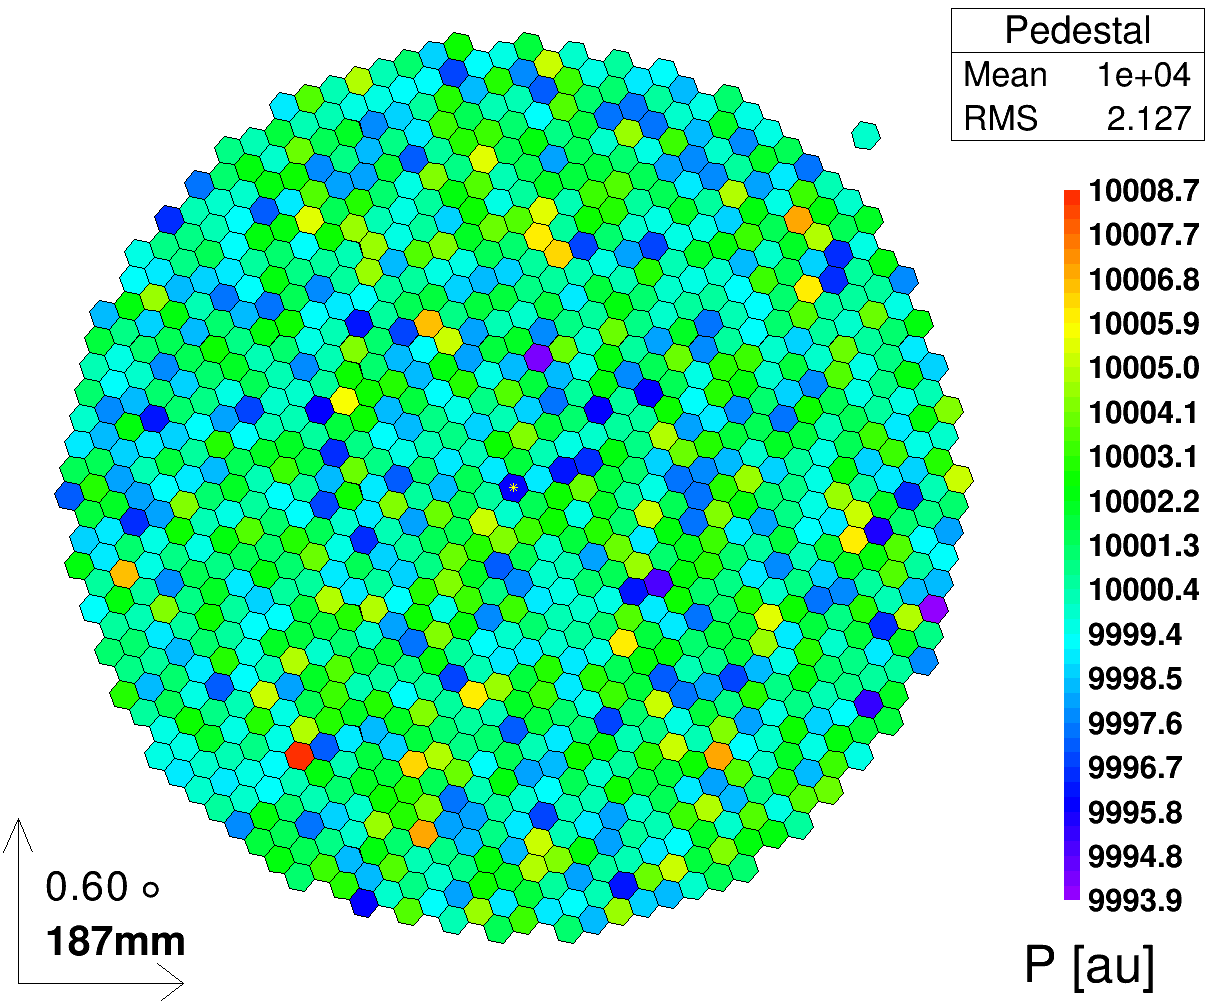
\includegraphics[width=0.6\textwidth]{./Plots/Pedestal_fertig.png}
    \caption{Darstellung eines simulierten Pedestal Events in der Kamera. Dargestellt ist der Pixelinhalt in [a.u.].}
    \label{Kamera-Bild-Pedestal}
\end{figure}

In der Realität sind Pedestal Events, Events mit zufälligem Trigger und ohne Puls und Calibration Runs sind Runs, die genommen werden, wobei die Calibration Box benutzt wird.
Diese Calibration Box befindet sich im Zentrum der Spiegel und verursacht kurze Lichtpulse mit konstanter Intensität in Richtung Kamera.


\subsection{Signalextraktion}
Ziel der Signalextraktion ist die Integration der Counts in der Pulsregion ohne Baseline.
Dafür gibt es verschiedene Methoden:
\begin{itemize}
 \item Fixed window: Mit dieser Methode wird an einer a priori bekannten Position, an der man den Cherenkovpuls erwartet, über eine bestimmte Länge integriert.
 \item Sliding window: Bei dieser Methode wird das Integrationsfenster so lange verschoben, bis man den Bereich gefunden hat, in dem das Signal am höchsten ist und integriert dort.
 \item Spline: Diese Methode beruht auf der Sliding Window-Methode, allerdings erfolgt die Integration mit Hilfe eines Polynoms.
\end{itemize}

Aktuell wird in MAGIC die Sliding Window Methode benutzt. Es wird in einem 60 time slice großen Bereich nach dem Pulse gesucht und dann über 6 time slices integriert ($\SI{3}{ns}$).

Nachdem man nun das Signal extrahiert hat, wird es noch von readout counts in Photoelektronen umgerechnet.

\subsection{Ankunftszeitbestimmung}
Die Ankunftszeit des Pulses wird als mittlere Time slice des integrierten Windows gewichtet mit dem Signal darin berechnet:

\begin{equation}
 t_{arrival}=\frac{\sum i s_i}{\sum s_i},\\
\end{equation}
\begin{center}
\tiny{mit $i$: time slice Nummer, $s_i$: Signal in slice i und der Summierung über 6 slices als Integrationsfenster.}
\end{center}


Eine typische Verteilung der Ankunftszeiten für einen Cherenkovschauer in Kamera ist in Abb.\ref{Kamera-Bild-ArrivalTimes} zu sehen.

\begin{figure}
    \centering
    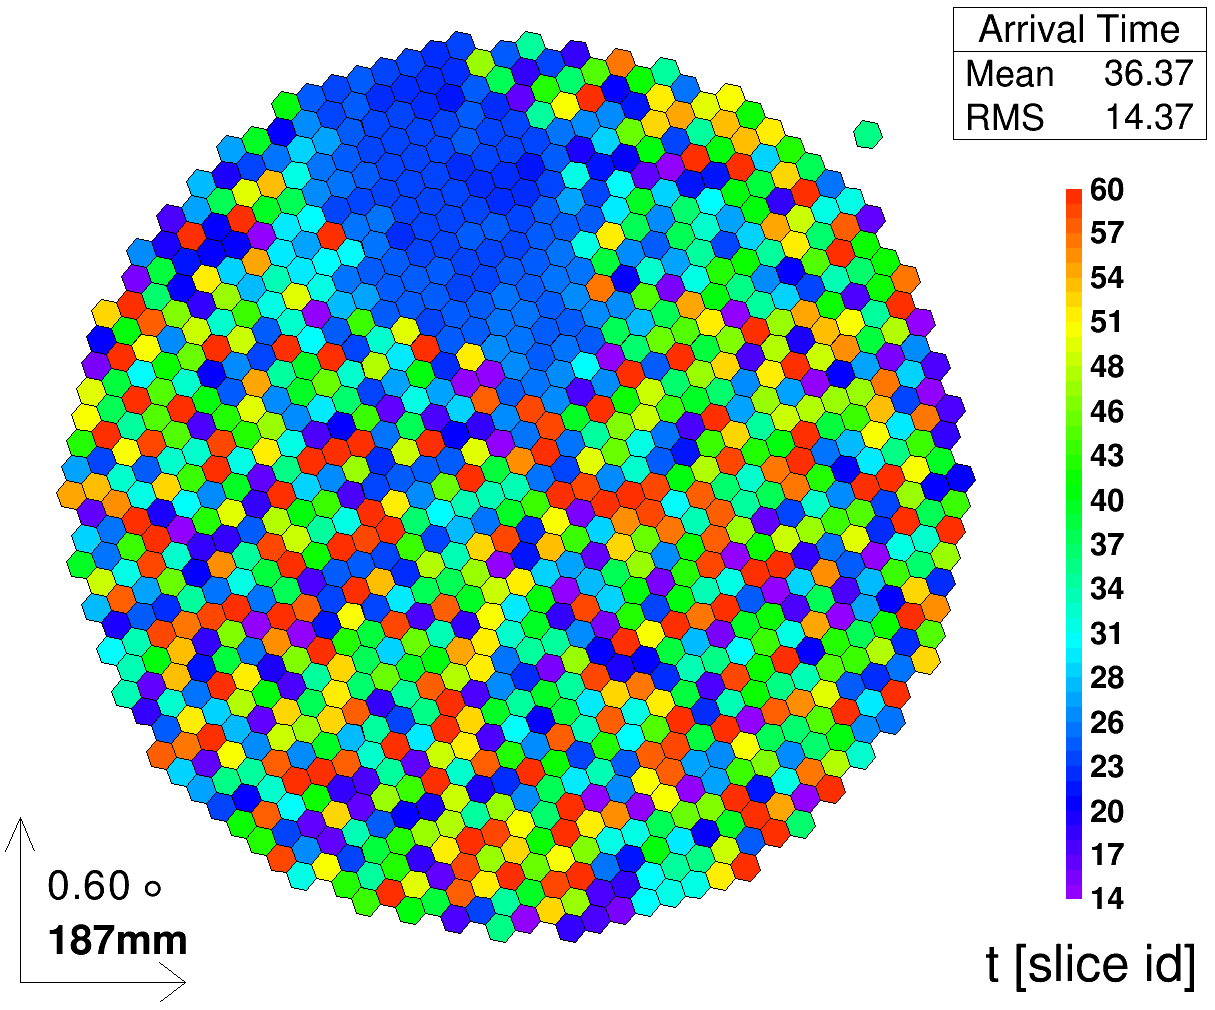
\includegraphics[width=0.6\textwidth]{./Plots/Signal_ArrivalTime_fertig.png}
    \caption{Darstellung der Ankunftszeiten eines Schauers in der Kamera. Dargestellt sind die Ankunftszeiten in time slices.}
    \label{Kamera-Bild-ArrivalTimes}
\end{figure}

\section{Star - Image Cleaning und Bildparametrisierung}

\subsection{Image Cleaning}
Im Programm \textit{Star} geschieht das Image Cleaning und die Parametrisierung des Schauerbildes.

Wird ein Event getriggert, werden die Signale der einzelnen Pixel gespeichert.
Sowohl Night Sky Background (NSB) als auch elektrisches Rauschen sind dann noch in dem Eventbild enthalten (siehe Abb.\ref{Kamera-Bild}).
Ziel des Image Cleanings ist es, das Bild von allem Background zu bereinigen, sodass nur noch das Signal vom eigentlichen Schauer überbleibt und eine robuste und stabile Parametrisierung dieses Schauerbildes durchgeführt werden kann.
Einerseits können Pixel, die nicht zum eigentlichen Schauer gehören und das Image Cleaning überleben, zu einer falschen Rekonstruktion führen, andererseits ist es zu vermeiden, dass zu viele Pixel im Cleaning wegfallen, da es so zu einem Signalverlust kommt, was ebenfalls zu einer schlechteren Rekonstruktion führen kann.
Also werden schlaue Algorithmen benötigt! 

Der einfachste und älteste Algorithmus ist das Absolute Image Cleaning.
Dabei wird nur die Photoncharge in den einzelnen Pixeln benutzt.
Es werden zwei Schwellwerte definiert für die Core ($Q_{Core}$) und die Boundary Pixel ($Q_{boundary}$).
Nun werden alle Pixel mit einer Photoncharge die größer als $Q_{Core}$ ist, ausgewählt.
Ein Pixel ist dann ein Corepixel, wenn er noch einen Nachbarn hat, welcher ebenfalls eine Photoncharge hat, die dieses Limit überschreitet.
Im zweiten Schritt werden alle Pixel mit direkten Nachbarn, die den vorherigen Schritt überlebt haben und eine Ladung größer als $Q_{boundary}$ haben, als boundary Pixel markiert.
Alle anderen Pixel fliegen raus.
Dieser Image Cleaning Algorithmus benutzt keine Zeitinformation und es wird damit keine niedrige Energieschwelle erreicht. 
Die verschiedenen Rauschlevel zwischen den Pixeln werden auch nicht berücksichtigt.

Eine Weiterentwicklung dieses Cleaningalgorithmus, welcher auch die Zeitinformationen benutzt, ist das Time Constrained Absolute Image Cleaning. 
Es funktioniert genauso wie das absolute Image Cleaning, allerdings wird die Ankunftszeit der Photonen zusätzlich berücksichtigt.

Eine weitere Entwicklung ist das Sum Image Cleaning, welches folgendermaßen funktioniert:
Es wird eine Zweier-, Dreier- oder Vierer-Kombination von Nachbarpixeln gesucht und deren Signale aufsummiert.
Ist das aufsummierte Signal über einer bestimmten Schwelle, werden die Ankunftszeiten in der Gruppe untereinander verglichen. 
Liegen diese nahe genug zusammen, werden die Pixel behalten, ansonsten verworfen.
Anschließend werden Nachbarpixel gesucht und deren Pixelinhalte und Ankunftszeiten betrachtet.

Beim dynamischen Sum Cleaning wird zusätzlich noch die Size, der Gesamtphotoneninhalt, eines Events mit berücksichtigt.

\subsection{Bildparametrisierung}
Die Bildparameter basieren auf den Hillas Parametern von 1985 [] und berücksichtigen die Verteilung der Photonen in den Pixeln, die zum gecleanten Event gehören.
Abb.\ref{Kamera-Bild-gecleant} zeigt ein gecleantes Event in der Kamera.

\begin{figure}
    \centering
    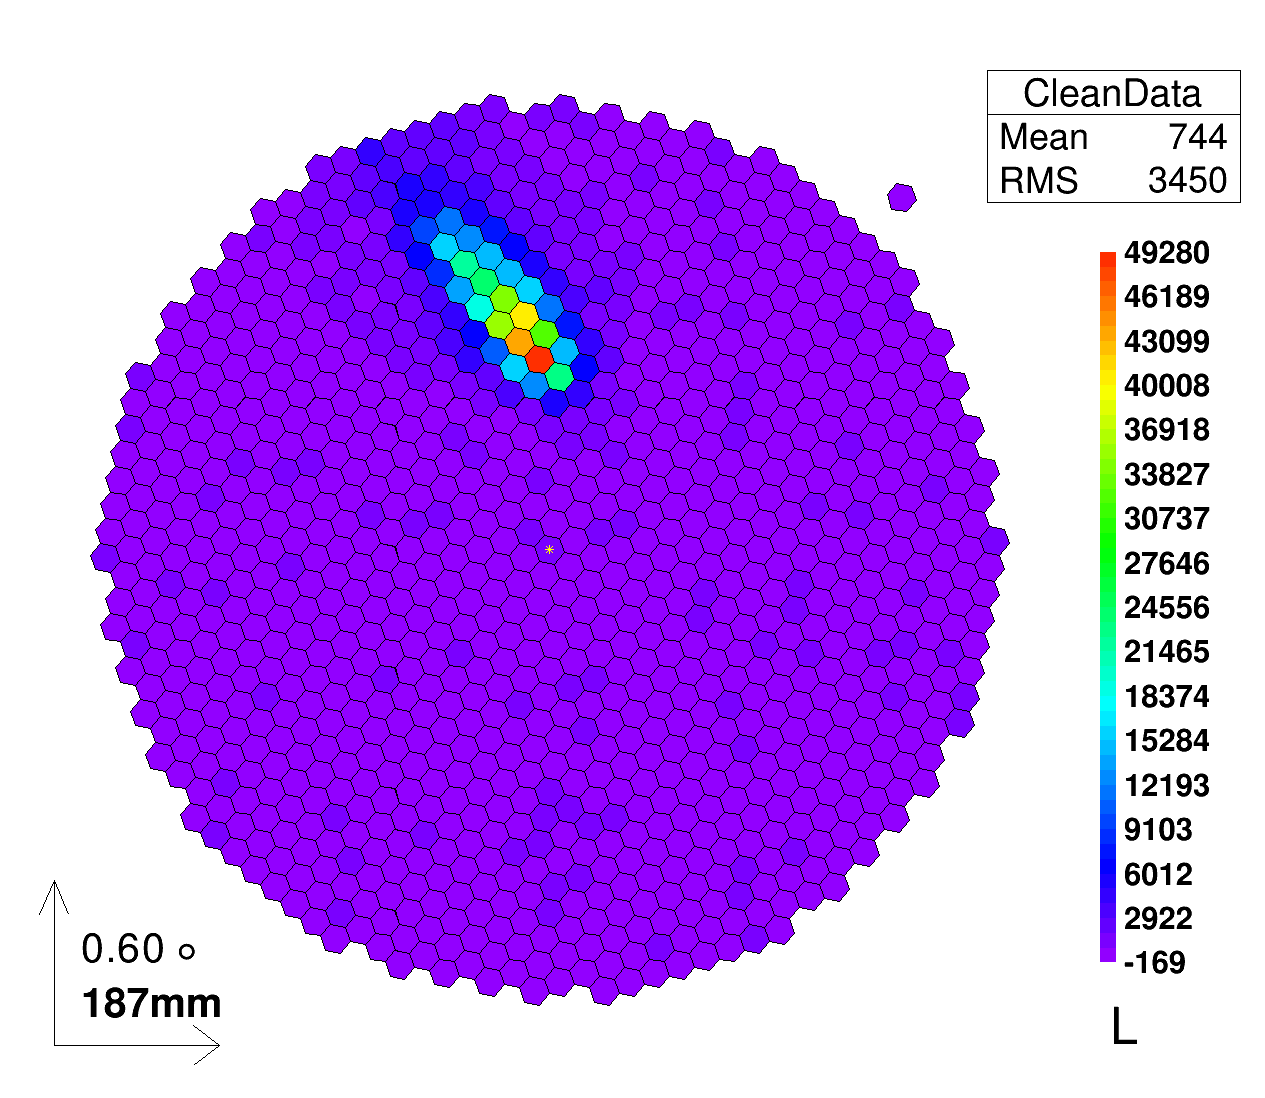
\includegraphics[width=0.6\textwidth]{./Plots/Signal_gecleant_fertig.png}
    \caption{Darstellung des gecleanten Events in der Kamera.}
    \label{Kamera-Bild-gecleant}
\end{figure}


Im Folgenden werden einige wichtige Bildparameter aufgelistet und beschrieben (vgl. Abb.\ref{CleaningBild}):

\begin{itemize}
 \item \texttt{size}: Die Gesamtzahl der Photoelektronen in einem ShowerImage wird als \texttt{size} bezeichnet. Für feste Zenitwinkel und Impactparameter ist diese Größe proportional zur gesuchten Primärteilchenenergie.
 \item \texttt{CoG} (Center of Gravity): Das Center of Gravity des Schauers bezeichnet die Position des gewichteten Mean Signals entlang der X- und Y-Achse in der Kamera. 
 X und Y sind die ersten Momente der Ladungsverteilung und werden \texttt{MeanX}, bzw. \texttt{MeanY} genannt.
 \item \texttt{Width}: Die halbe Breite der kleinen Halbachse der an den Schauer gefitteten Ellipse wird als \texttt{Width} bezeichnet. 
 Mit Hilfe dieses Paramters lassen sich Aussagen über die transversale Ausbreitung des Schauers und damit auch über den Ursprung des Schauers (hadronisch oder elektromagnetisch) treffen. 
 Dieser Parameter ist somit ein guter Trennparameter.
 \item \texttt{Length}: Die halbe Länge der großen Halbachse wird mit dem Parameter \texttt{Length} bezeichnet.
 Dieser Parameter trifft eine Aussage über die longitudinale Entwicklung des Schauers und ist im Allgemeinen größer für Hadroninduzierte Schauer als für Gammainduzierte Schauer.
 \item \texttt{Conc-n}: Der Anteil der Photoelektronen, welche in den n hellsten Pixeln enthalten sind, wird als \texttt{Conc-n} bezeichnet.
 Damit ist es möglich, die Kompaktheit des Schauermaximums zu beschreiben. 
 Bei Gamma-Schauern ist die Region sehr kompakt.
 \item \texttt{Leakage}: Dieser Parameter beschreibt den Anteil des Signals im äußeren Kameraring im Vergleich zur totalen Image Size.
 Es ist möglich mit diesem Parameter den Signalverlust zu beschreiben und zu entscheiden, ob der Schauer überhaupt noch vernünftig rekonstruiert werden kann.
 \item \texttt{M3Long}: Dieser Parameter ist das dritte Moment entlang der großen Halbachse und beschreibt die Asymmetrie des Schauers.
 Es lässt sich damit also auf die Herkunftsrichtung des Schauers schließen. 
 \texttt{M3Long} ist positiv wenn der Schauerschwerpunkt in Richtung des Kamerazentrums liegt, ansonsten negativ.
 \item \texttt{Number\_of\_Islands}: Wie der Name schon sagt wird mit diesem Parameter die Anzahl der Inseln, die nach dem Cleaning übergeblieben sind, bezeichnet. 
 Je größer dieser Wert ist, umso mehr Inseln sind noch vorhanden und umso wahrscheinlicher ist der Schauer hadronischen Ursprungs.
\end{itemize}

\begin{figure}
    \centering
    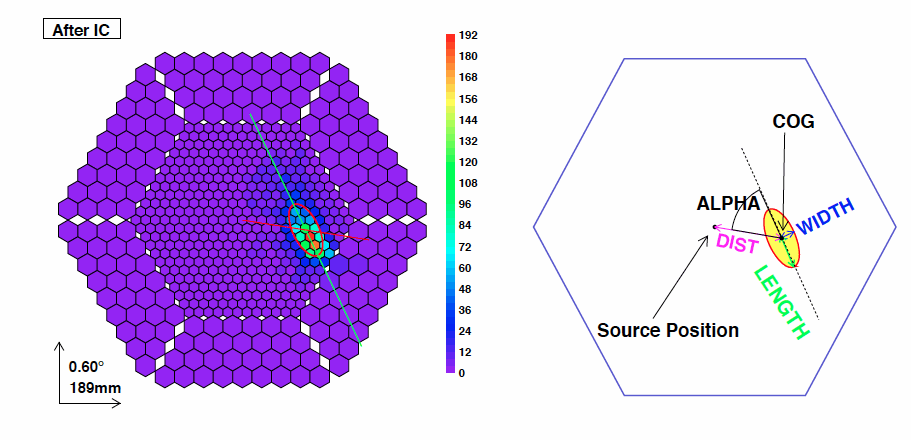
\includegraphics[width=0.9\textwidth]{./Plots/CleaningBild.png}
    \caption{Beispielhafte Darstellung eines bereinigten Bildes und einiger Bildparameter in der alten MAGIC-Kamera.}
    \label{CleaningBild}
\end{figure}

Abgesehen von diesen Bildparametern gibt es auch noch Parameter, die zu einem bestimmten Referenzpunkt, z.B. der Quellposition, in der Kamera berechnet werden. 

\begin{itemize}
 \item \texttt{Alpha}: \texttt{Alpha} bezeichnet den Winkel zwischen der großen Halbachse der Ellipse und der Linie vom CoG zum Referenzpunkt.
 Dieser Parameter beinhaltet eine große Gamma-Hadron-Trennkraft, da gamma-induzierte Schauer zur Quellposition in der Kamera zeigen und somit alpha klein ist.
 Hadroninduzierte Schauer sind isotrop in der Kamera verteilt.
 \item \texttt{Dist}: \texttt{Dist} ist der Abstand vom CoG zum Referenzpunkt und bietet Informationen über den Abstand von Schauermaximum zur Teleskopachse.
\end{itemize}

Außerdem gibt es noch einige Parameter, die die Ankunftszeit der Cherenkovphotonen zusätzlich berücksichtigen, wie z.B.:

\begin{itemize}
 \item \texttt{TimeGradient}: Der \texttt{TimeGradient} bietet ein Zeitprofil eines Events.
 Die Pixel werden auf die Hauptachse projiziert.
 Dann wird ein Graph der Ankunftszeiten der einzelnen Pixel erstellt und mit einer linearen Funktion gefittet.
 Die Steigung dieser gefitteten Geraden wird dann als Time Gradient bezeichnet.
 \item \texttt{TimeRMS}: So wird der Arrivaltime Spread der Cherenkovphotonen in den Bildpixeln bezeichnet:
 
\begin{equation}
 Time-RMS=\sqrt{\sum_{i=1}^k (t_i-t_{mean})^2}
\end{equation}
 \begin{centering}
  \tiny{mit k:Anzahl der Pixel, $t_i$: Ankunftszeit im i-ten Pixel und $t_mean$:mittlere Ankunftszeit}
 \end{centering}


\end{itemize}

Mit Hilfe dieser Bildparameter und der stereoskopischen Bildparameter kann dann im Folgenden die Gamma-Hadron-Separation durchgeführt werden.


\section{Superstar - Stereoskopische Rekonstruktion der Schauer}
Mit Hilfe des Programms Superstar geschieht die stereoskopische Rekonstruktion der Schauerparameter.

Der Kreuzungspunkt der beiden Hauptachsen der projizierten Bilder des Schauers in den beiden MAGIC-Kameras erlaubt einen Rückschluss auf die Ursprungsrichtung des Schauers.
Anhand geometrischer Überlegungen können die Schauerachse und der Core Impact Punkt auf der Erde, sowie die beiden individuellen Impactparameter der Teleskope bestimmt werden (siehe Abb.\ref{Superstar}).

Auch die Höhe des Schauermaximums wird in Superstar bestimmt.

\begin{figure}
    \centering
    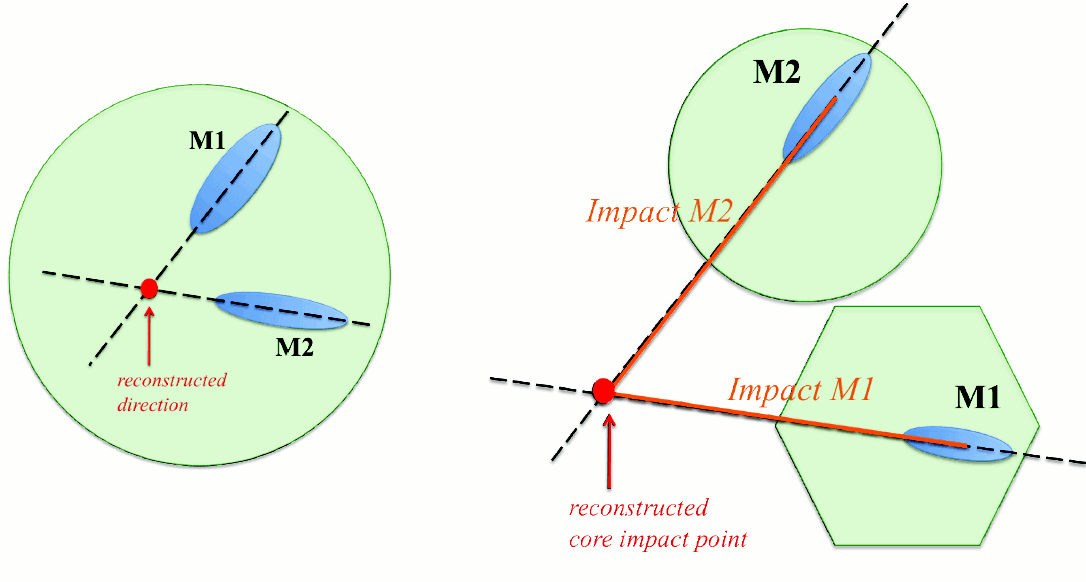
\includegraphics[width=0.9\textwidth]{./Plots/Superstar.png}
    \caption{Rekonstruierte Richtung und rekonstruierter Core Impact Punkt}
    \label{Superstar}
\end{figure}

Des Weiteren werden noch der Cherenkov-Radius und die Cherenkovlichtdichte bestimmt.

Der Cherenkovradius ist der Radius am Boden, der von einem 87MeV Elektron,welches in Schauerrichtung fliegt, in der Höhe des Schauermaximums produziert wird.

Die Cherenkovlichtdichte ist die Lichtdichte am Boden, die von einem 1m langen Track eines 86MeV Elektrons im Schauermaximum produziert wird, welches ebenfalls in Schauerrichtung fliegt.

%Alle mit Superstar geometrisch berechneten Parameter werden im root Container MStereoPar gespeichert:

% \begin{itemize}
%  \item fCoreX / fCoreY: berechnete CorePosition auf dem Boden
%  \item fDirectionAz/fDirectionDec/fDirectionRA: berechneter Azimut, bzw. Deklination und Rektaszension der Schauerachse
%  \item fM1Impact: berechneter Impactparameter für MAGIC 1, bzw. 2
%  \item fMaxHeight: berechnete Höhe des Schauermaximums
% \end{itemize}

% \begin{figure}
%     \centering
%     
\includegraphics[width=0.9\textwidth]{./Plots/Superstar.jpg}
%     \caption{Stereokacke.}
%     \label{Jobmanager}
% \end{figure}



\section{Automatische MC-Produktion hier in Dortmund geht so}

Die Monte Carlo Produktion an der TU Dortmund geschieht automatisiert mit Hilfe von bash-Skripten und einer mysql-Datenbank siehe \ref{Jobmanager}.

\begin{figure}
    \centering
    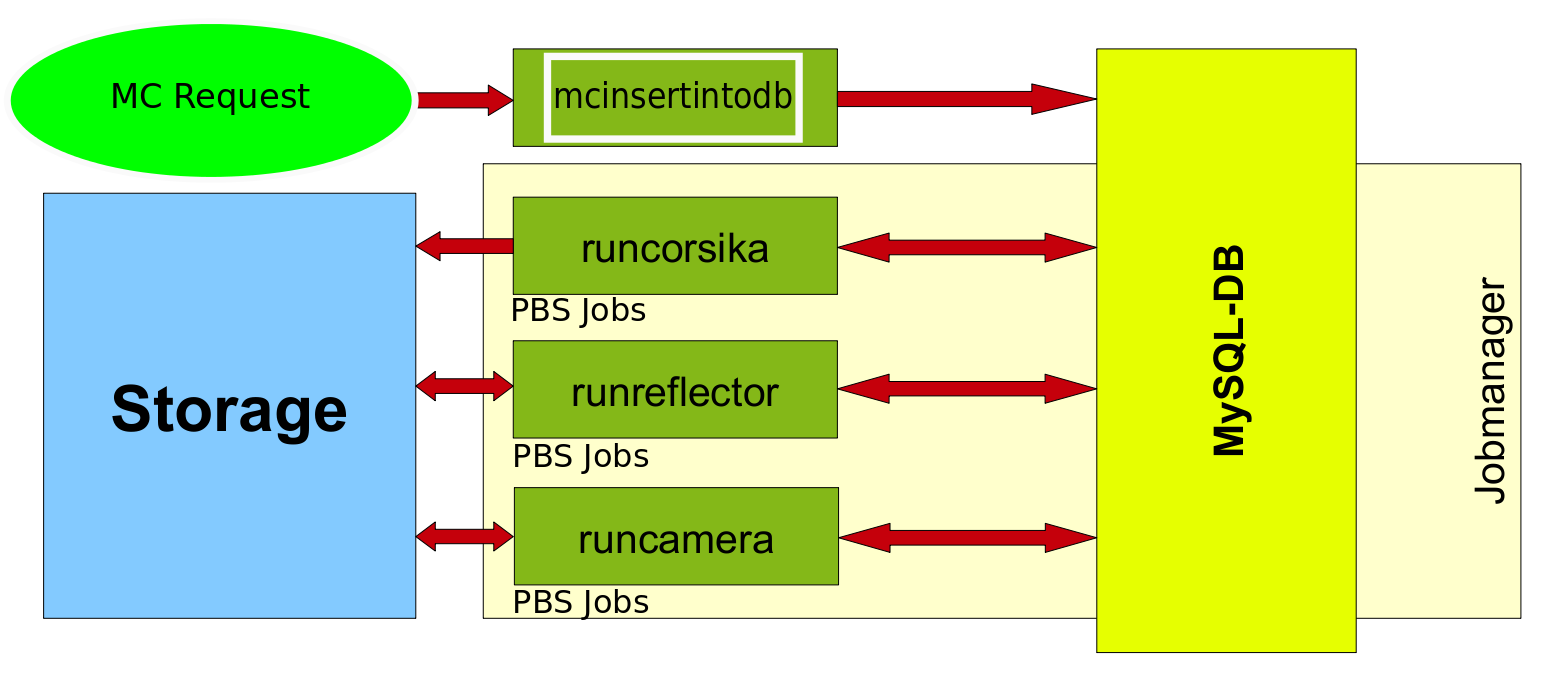
\includegraphics[width=0.9\textwidth]{./Plots/Jobmanager.png}
    \caption{Schematische Darstellung der automatischen MC Produktionskette.}
    \label{Jobmanager}
\end{figure}


Bei einer neuen Anfrage für MC Daten werden mit Hilfe des mcinsertintodb-Skripts die für die gewünschte Produktion benötigten Inputcard-Parameter in die Datenbank geschrieben.
Im Hintergrund läuft die ganze Zeit das jobmanager-Skript, welches überprüft, ob in der Datenbank ein neuer Auftrag (Job) eingegangen sind.
Falls dies der Fall ist, startet das jobmanager-Skript automatisch das runcorsika-Skript, welches wiederum Corsika für diesen neuen Job mit den gewählten Einstellungen startet.
Sobald Corsika beendet ist, wird dies in die Datenbank geschrieben, sodass das nächste Programm in der Monte Carlo-Kette gestartet werden kann.
Für das nächste Programm in der Kette sind alle benötigten Parameter schon bei der Inauftraggabe des Jobs in der Datenbank gespeichert worden.
Also wird Reflector mit Hilfe des runreflector-Skripts gestartet und nach Beendigung und Eintragen in die Datenbank auch Camera.

Nach dem erfolgreichen Durchlauf eines kompletten Jobs  bestehend aus 1000-2000 Runs mit je 1000 Events werden die generierten MC Daten nach jedem Programmdurchlauf auf dem Cluster gespeichert.
Sobald die Simulationskette für einen Job beendet wurde, wird dies wiederum in die Datenbank eingetragen.

Die Kalibrationskette, die aus den Programmen Sorcerer, Star und Superstar besteht wird analog durchgeführt:
Mit Hilfe der run-Skripte werden die Programme gestartet und nach erfolgreichem Durchlauf die Daten gespeichert.

\subsection{Datenbank}
Wie oben beschrieben, werden die wichtigsten Inputparameter und die Pfade zu den MCs in einer mysql-Datenbank gespeichert.
Diese Datenbank beinhaltet die Tabellen in Tab.\ref{MYSQL_Tabellen}:

\begin{table}[!h]
\centering
\caption{Auflistung der Tabellen, die in der Datenbank existieren....Hmpf!}
\label{MYSQL_Tabellen}
\begin{tabular}{l}
  \toprule
  Tabellen\\
  \midrule
  AtmosphericModel           \\
  AzimuthBinning             \\
  FADCType                   \\
  M1CalibrationProcessStatus \\
  M1CameraCopytoGridStatus   \\
  M1StarCopytoGridStatus     \\
  M2CalibrationProcessStatus \\
  M2CameraCopytoGridStatus   \\
  M2StarCopytoGridStatus     \\
  MCCalibrationRuns          \\
  MCCameraRunData            \\
  MCCorsikaRunData           \\
  MCJobs                     \\
  MCPedestalRuns             \\
  MCReflectorRunData         \\
  MCRunData                  \\
  MCRunProcessStatus         \\
  MCStatistics               \\
  MCSuperstarProcessStatus   \\
  MCUserID                   \\
  MarsVersion                \\
  ObservationMode            \\
  ParticleType               \\
  Source                     \\
  ZenithBinning   	     \\
  \bottomrule
\end{tabular}
\end{table}

% +----------------------------+
% | $Tables_in_magicprod$        |
% +----------------------------+
% | AtmosphericModel           |
% | AzimuthBinning             |
% | FADCType                   |
% | M1CalibrationProcessStatus |
% | M1CameraCopytoGridStatus   |
% | M1StarCopytoGridStatus     |
% | M2CalibrationProcessStatus |
% | M2CameraCopytoGridStatus   |
% | M2StarCopytoGridStatus     |
% | MCCalibrationRuns          |
% | MCCameraRunData            |
% | MCCorsikaRunData           |
% | MCJobs                     |
% | MCPedestalRuns             |
% | MCReflectorRunData         |
% | MCRunData                  |
% | MCRunProcessStatus         |
% | MCStatistics               |
% | MCSuperstarProcessStatus   |
% | MCUserID                   |
% | MarsVersion                |
% | ObservationMode            |
% | ParticleType               |
% | Source                     |
% | ZenithBinning              |
% +----------------------------+

Die Tabelle MCJobs bietet eine Übersicht über alle Jobs. 
Enthalten sind in dieser Tabelle u.a. die JobID, die jedem Job individuell zugewiesen wird, die erste und letzte Runnummer eines Jobs, wann der Job gestartet wurde, wann Camera und Star beendet wurden und den Pfad zu den Daten.\newline
Die Tabellen M1CalibrationProcessStatus und M2CalibrationProcessStatus enthalten ebenfalls die JobID, und die Zeitpunkte wann Camera, Calibration und Star beendet worden. 
Des Weiteren kann man den Startzeitpunkt und den Zeitpunkt eines Abbruchs des Jobs, sowie den zugehörigen Fehlercode sehen, der Rückschlüsse über die Ursache des Fehlers bietet.

In den Tabellen MCCorsikaRunData, MCReflectorRunData und MCCameraRunData kann man die wichtigsten Inputparameter für die jeweiligen Programme sehen.

Die Tabelle MCRunData bietet eine Übersicht über die Runnummern, die innerhalb der einzelnen Programme verteilt wurden. 
So gehört zu jeder Runnumber eine CorsikaRunNumber, eine ReflectorRunNumber und eine CameraRunNumber.
Also bietet ein Job mit 2000 x 1000 Events Platz für 2000 RunNummern pro Programm.

Die Tabelle MCRunProcessStatus ist eine Übersichtstabelle über die Zeitpunkte zu denen die jeweiligen Inputcards geschrieben und die Programme Corsika, Reflector und Camera beendet wurden.

Die gleiche Tabelle gibt es auch noch für Superstar. 


\subsection{LiDO}
Die Monte Carlo-Produktion wird an der TU Dortmund vorwiegend auf dem LiDo-Cluster (Linux Cluster Dortmund) durchgeführt. 
Für die gesamte MAGIC Kollaboration werden hier die Gamma-MCs produziert und gespeichert.

Dafür stehen insgesamt 3328 CPUs und 215TB Speicher auf dem LiDO zur Verfügung.
Die Struktur des Clusters lässt sich Abb.\ref{LiDo} entnehmen.

\begin{figure}[!h]
    \centering
    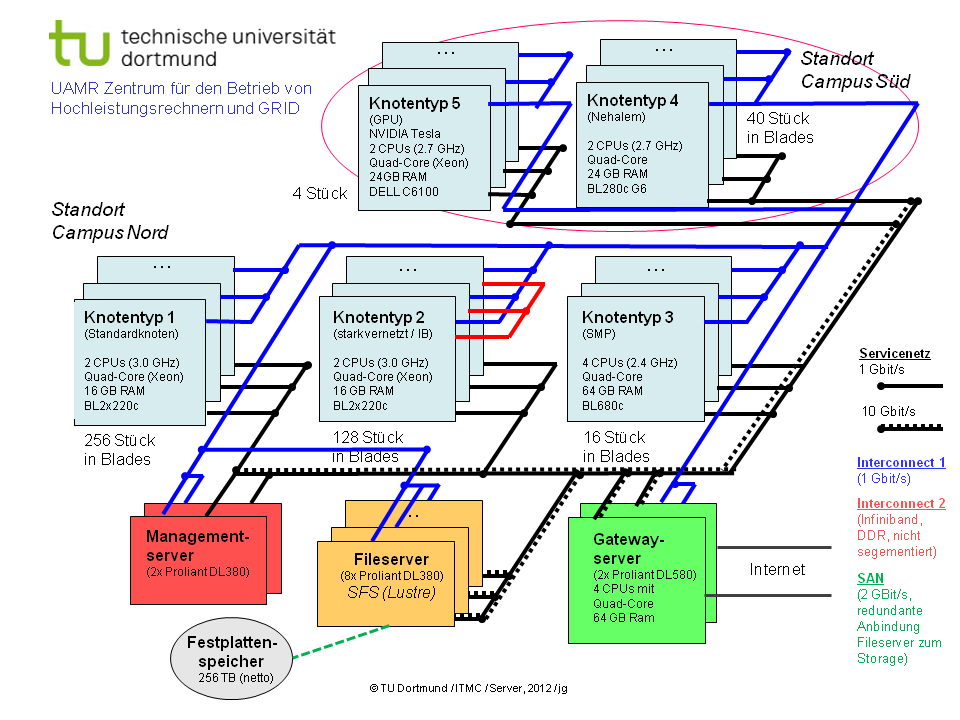
\includegraphics[width=0.9\textwidth]{./Plots/LiDO.png}
    \caption{Schematische Darstellung des Rechenclusters LiDO.}
    \label{LiDo}
\end{figure}


Über die beiden Gateway-Server erhält man Zugriff auf die Rechenknoten und den Speicher.
Wie in Abb.\ref{LiDo} zu sehen ist, gibt es verschiedene Knotentypen, die sich in der Zahl der maximalen Jobs pro Queue und Nutzer unterscheiden und über ein Queuingsystem erreichbar sind:

\begin{itemize}
 \item Die ib-Knoten sind für parallele Jobs reserviert, die die Infiniband interconnect nutzen
 \item eth-Knoten: Auf diesen Knoten werden serielle und parallele Jobs gerechnet, die die GigabitEthernet Connection nutzen
 \item quad-Knoten: Für Anforderungen an viel Speicher oder parallele OpenMP/Shared Memory Jobs werden die quad Knoten genutzt
 \item GPU: Rechnungen auf Graphikkarten finden hier statt.
 \item nehalem: neue Testknoten mit einer maximaler Walltime von 96h und mehr Arbeitsspecher als die eth-Knoten
\end{itemize}

Die meisten Knoten haben drei verschiedene Queues, die sich in ihrer maximal zur Verfügung stehenden Walltime unterscheiden.
Es gibt als die short Queues (eth, ib, quad) mit einer maximalen Walltime von 1h, die medium Queues (eth, eth\_nhm, ib, quad) mit einer Walltime von 8h und die long Queues mit einer maximalen Walltime von 48h. 
Falls es doch mal länger dauern sollte, gibt es noch die ultralong Queue (eth) mit einer maximalen Walltime von 2688h.
Um also einen Job zu starten, gibt man den benötigten Speicher und eine maximale Walltime an und submittet den Job in das Queuingsystem.

Für die MAGIC MC Produktion werden die eth-Knoten benutzt und pro Run 1000 Corsika Events produziert und weiter prozessiert. 
Ein Standardjob von 2Mio Corsika Events wird also in 2000 Runs mit je 1000 Events darin aufgeteilt und somit 2000 Runs nacheinander an das Queuingsystem submitted.


Im Moment wird auf dem LiDO folgendes Speichervolumen für die Daten nach den verschiedenen Programmen genutzt:

\begin{table}[h!]
    \centering
    \caption{Soviel Speichervolumen wird auf dem LiDo benutzt}
    \label{tab:bsp}
    \begin{tabular}{ccccccc}
        \toprule
        Programm & Corsika & Reflector & Camera & Sorcerer & Star & Superstar\\
        \midrule
        Speichervolumen [TB] & 49 & 36 & 9 & 1.3 & 0.5 & 0.5\\
        \bottomrule
    \end{tabular}
\end{table}

Alternativ kann auch noch der PhiDo Cluster für Testproduktionen, bzw. früher für dezidierte Protonsimulationen benutzt werden. 
Dieser Cluster stellt 1200 CPUs und 200TB(ZAHLEN NACHGUCKEN) Speicher zur Verfügung, hat allerdings auch eine größere Auslastung, was dazu führt, dass eine komplette Produktion wesentlich länger dauert.



\subsection{Wenn die MC fertig sind...Keine Ahnung, ob das interessant ist...}
Sobald eine Produktion an MCs fertig gerechnet ist, werden die Daten ins Grid kopiert.
Das heißt im Moment werden sie auf Computer im Rechenzentrum in Spanien PIC kopiert, welche zum Grid gehören und dort gespeichert, sodass sie immer über eine Internetseite erreichbar sind.
Die Struktur, in der die MCs gespeichert sind, ist so: 

MonteCarlo / Chipsatz der beiden Teloskope / PSF und Mirror fraction / Teilchentyp / Zenitbereich / Observationsart / Standart der Software / Level der Prozessierung / Versionsnummer \newline

\url{http://data.magic.pic.es/Data/MonteCarlo_Stereo/M1_DRS4_1039_M2_DRS4_1039/M1_PSF10.1_MF0.60_M2_PSF8.6_MF0.66/gammas/za05to35/ringwobble/std20140317/superstar/mc_v07/}


%Achten Sie bei ihren Plots auf ausreichend große Achsenbschriftungen, ausreichende Schriftdicken und gut unterscheidbare Farben.
% Im Idealfall haben Sie im Plot und der Arbeit die gleiche Schriftgröße und Schriftart.
% Dies lässt sich durch Erstellen des Plots in der korrekten Größe und einbinden mit dem optionalen Argument \texttt{scale=1} erreichen. Ein Beispiel sehen Sie in Abbildung \ref{fig:bsp}.

% Nutzen Sie wenn möglich Vektorgrafiken (pdf) und nur in Ausnahmen Rastergrafiken wie .png oder .jpg.
% Setzen Sie Punkte hinter Abbildungsunterschriften.
% 
% \begin{figure}[!h]
%     \centering
%     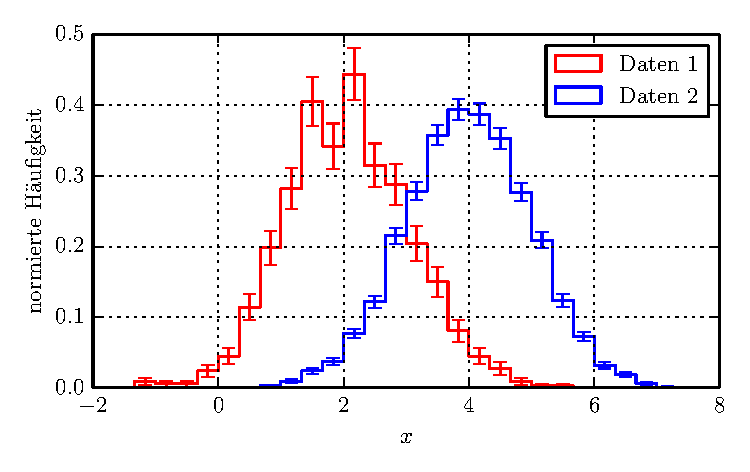
\includegraphics[scale=1]{./Plots/Histogramm.pdf}
%     \caption{Ein Histogramm mit Fehlerbalken für zwei Datensätze, Schriftgröße und -art entsprechen der des Dokuments.}
%     \label{fig:bsp}
% \end{figure}
% 
% \section{Tabellen}
% 
% Tabellen sollten so einfach wie möglich aufgebaut sein, verzichten Sie auf zu viele Linien. In fast allen Fällen reichen drei horizontale Linien aus, jeweils über und unter der Tabelle und zwischen den Spaltenüberschriften und der eigentlichen Tabelle.
% 
% Das Paket \texttt{booktabs} stellt hierfür die Befehle \verb_\toprule_, \verb_\midrule_ und 
% \verb_\bottomrule_ zur Verfügung.
% Das Paket \texttt{siunitx} stellt eine extrem mächtige neue Spalteneinstellung bereit: \texttt{S}, mit ihr können Zahlen und Einheiten sehr sauber und gut ausgerichtet gesetzt werden.
% 
% Diese Vorlage geht von Tabellenüberschriften aus, möchten Sie dagegen Tabellenunterschriften entfernen Sie das entsprechende optionale Argument für die Dokumentenklasse in der Präambel.
% 
% Eine Beispiel ist Tabelle \ref{tab:bsp}.
% 
% \begin{table}[!h]
%     \centering
%     \caption{Beispieltabelle mit willkürlichen Werten, für die Zahlenwerte wurde die S-Option aus SIunitx verwendet, für die Einheitenspalte die s-Option.}
%     \label{tab:bsp}
%     \begin{tabular}{l S[table-format=3.2] S[table-format=3.2(2)] s}
%         \toprule
%         Variable    & {Theoriewert} & {gemessener Wert} & {Einheit}\\
%         \midrule
%         Druck       & 1,23      & 1,31(5)   & \pascal \\
%         Temperatur  & 273,15    & 273,5(2) & \kelvin \\
%         \bottomrule
%     \end{tabular}
% \end{table}
